\section{Resultados y análisis}

\subsection{Generador Termoeléctrico}
Una vez realizada la regresión de los datos de $P_open$ se usa la relación lineal obtenida en el rango de temperaturas que en el que se midieron los demás parámetros. Es decir, se obtuvo $P_{open} = P_{open}(\Delta T)$ y se evaluó en el rango de $\Delta T = 0 - 40 \si{\celsius}$
\begin{figure}[ht]
    \centering
    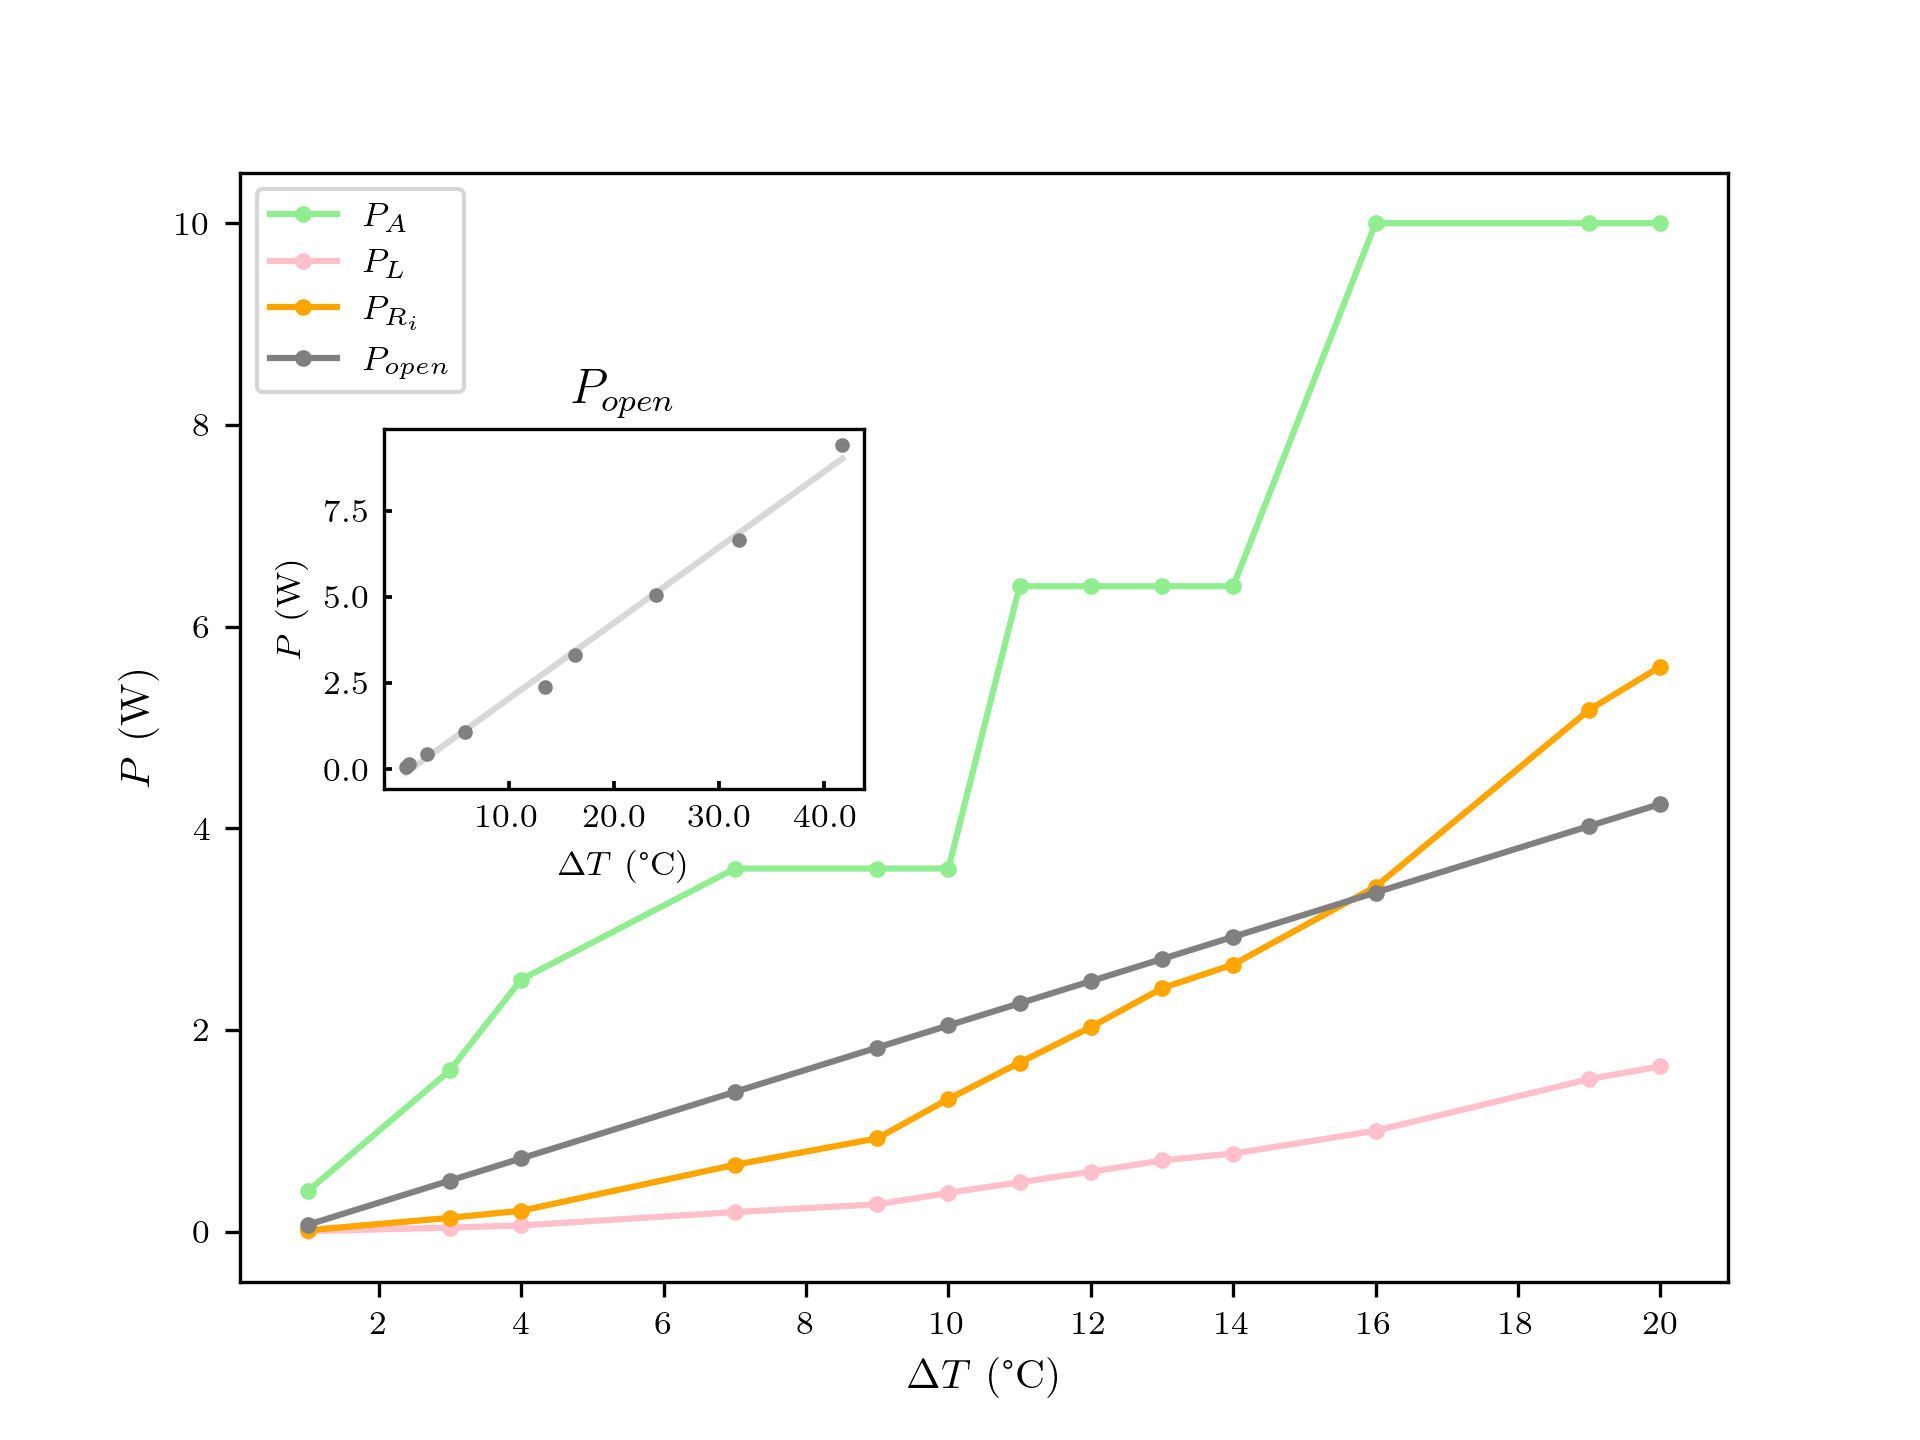
\includegraphics[width = 0.8\linewidth]{img/gen_powers.png}
    \caption{Potencias medidas para el módulo térmico usado como generador térmico. Los datos de $P_{open}$ se midieron en un rango distinto de temperatura y con una escala más fina (décimas de grado).}
    \label{fig:powers}
\end{figure}

% etas

\begin{figure}[ht]
    \centering
    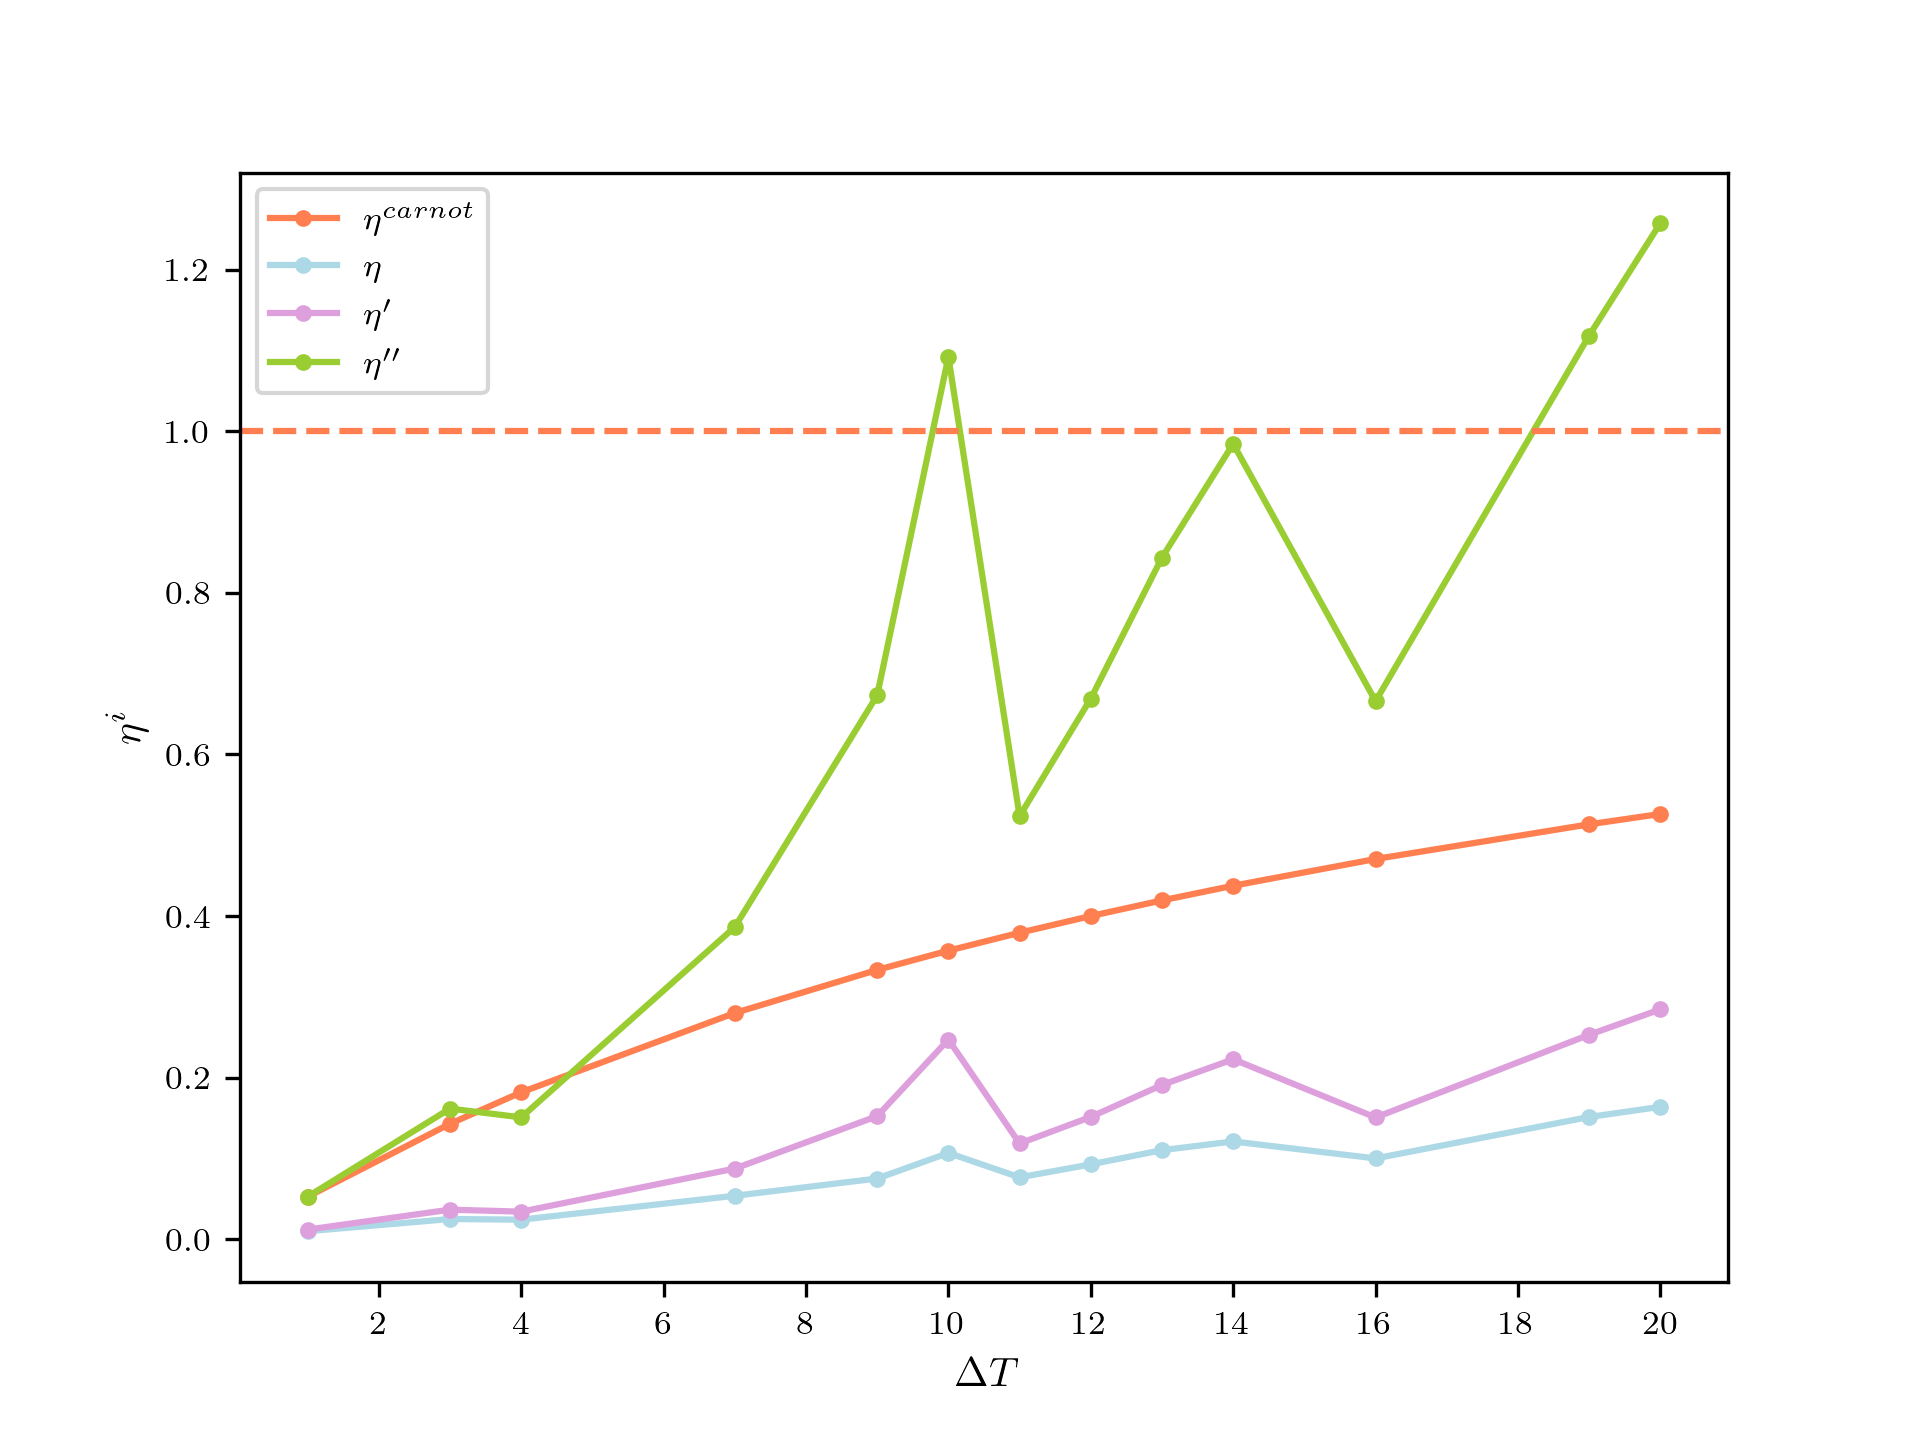
\includegraphics[width = 0.8\linewidth]{img/gen_etas.png}
    \caption{Comparación de las diferentes eficiencias calculadas como función de la diferencia de temperatura}
    \label{fig:etas}
\end{figure}

\subsection{Refrigerador}

\begin{figure}[ht]
    \centering
    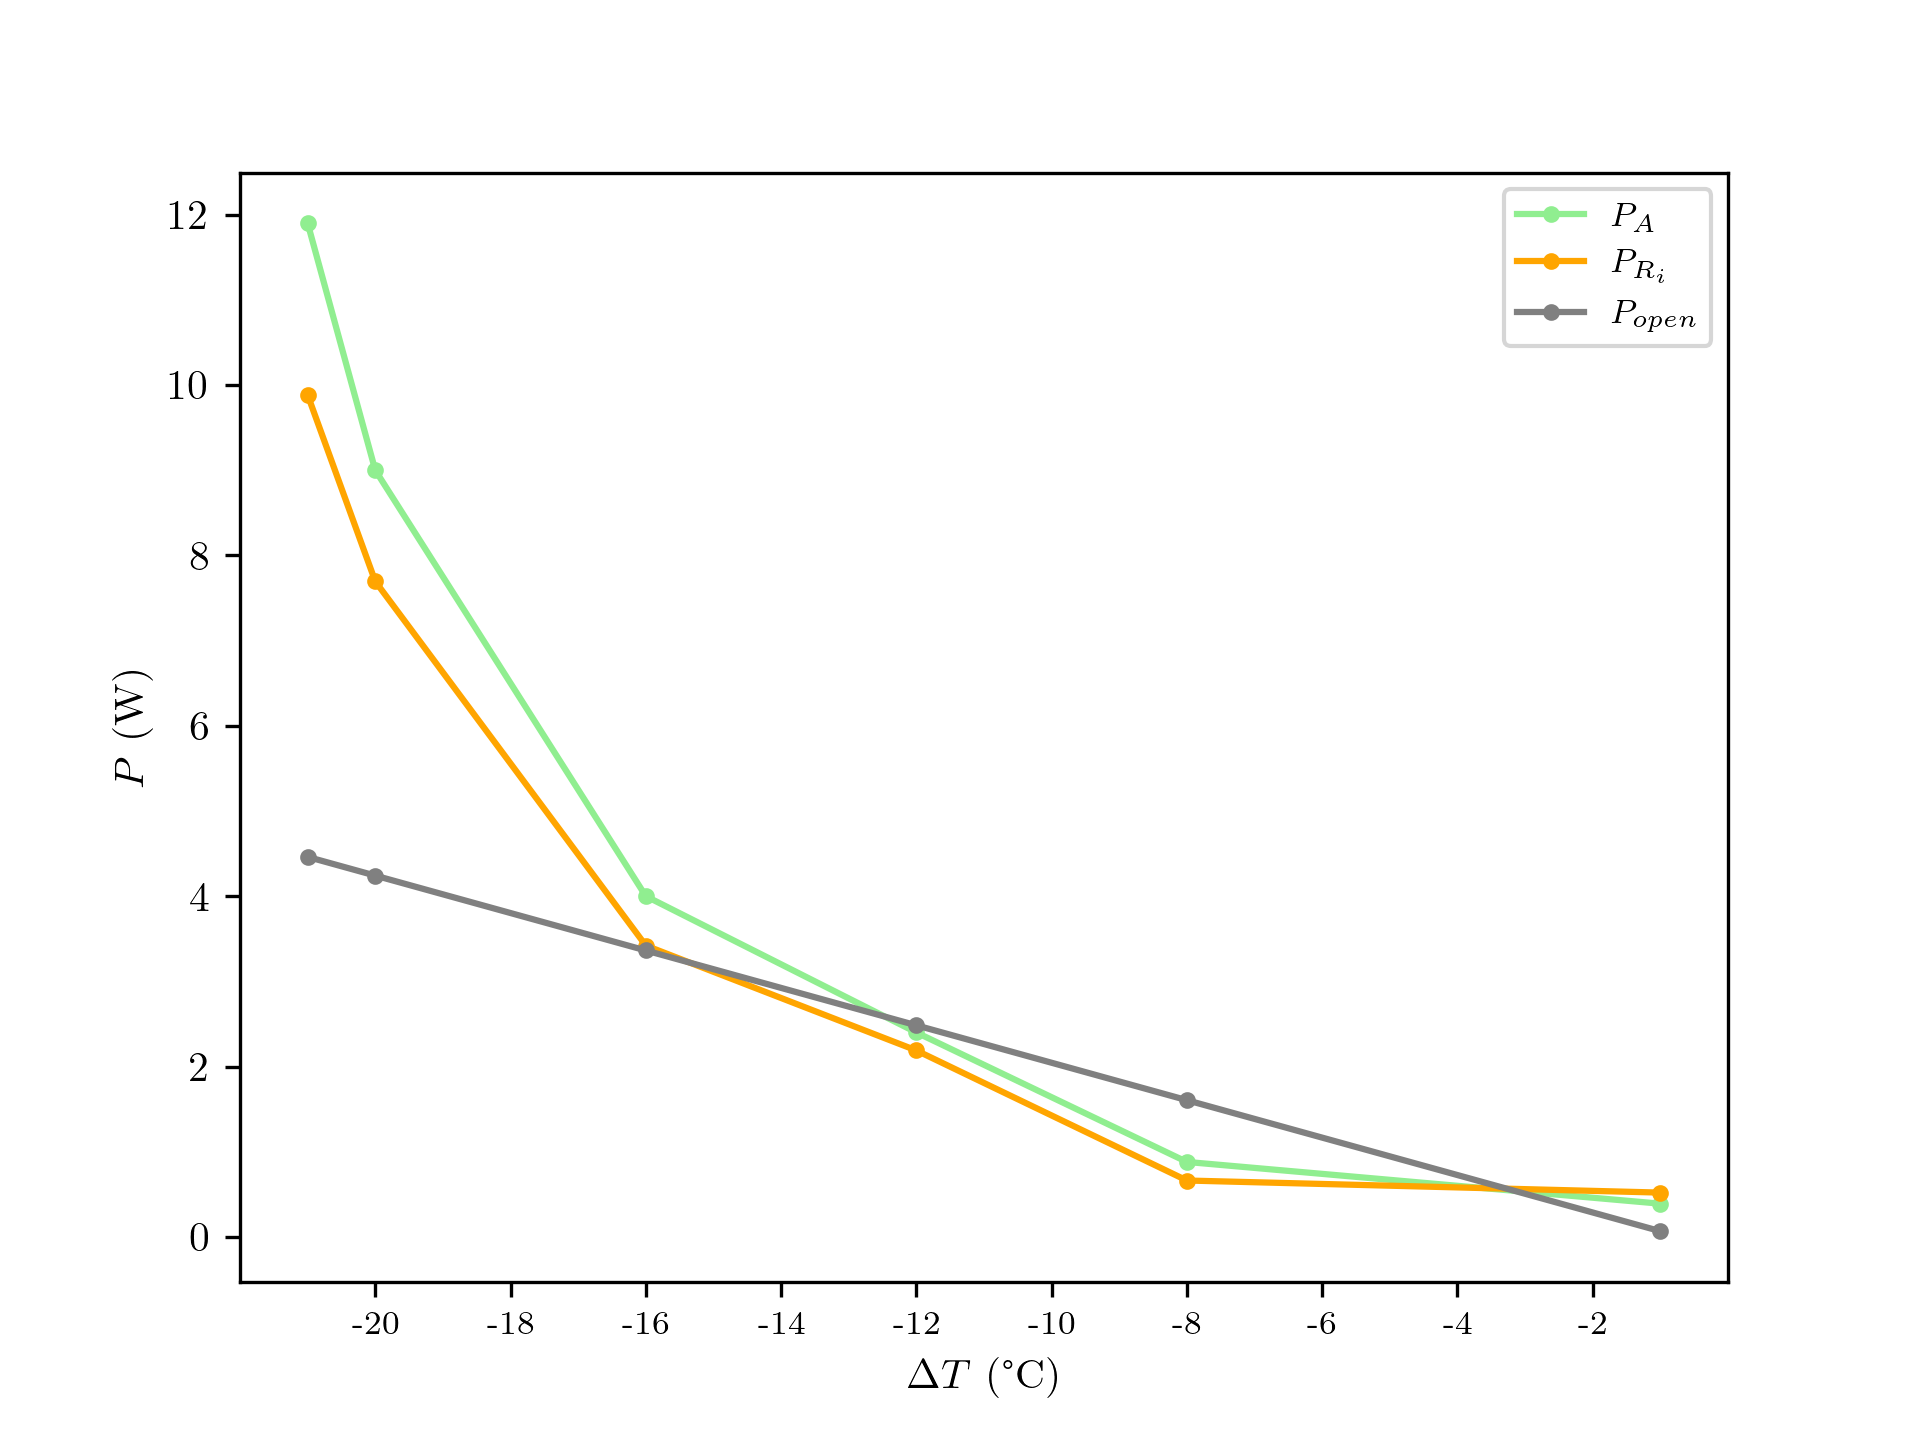
\includegraphics[width = 0.8\linewidth]{img/refri_powers.png}
    \caption{Potencias medidas para el módulo térmico usado como refrigerador. Se usa la misma recta de $P_{open}$ usada en el montaje anterior.}
    \label{fig:refri_powers}
\end{figure}

\begin{figure}[ht]
    \centering
    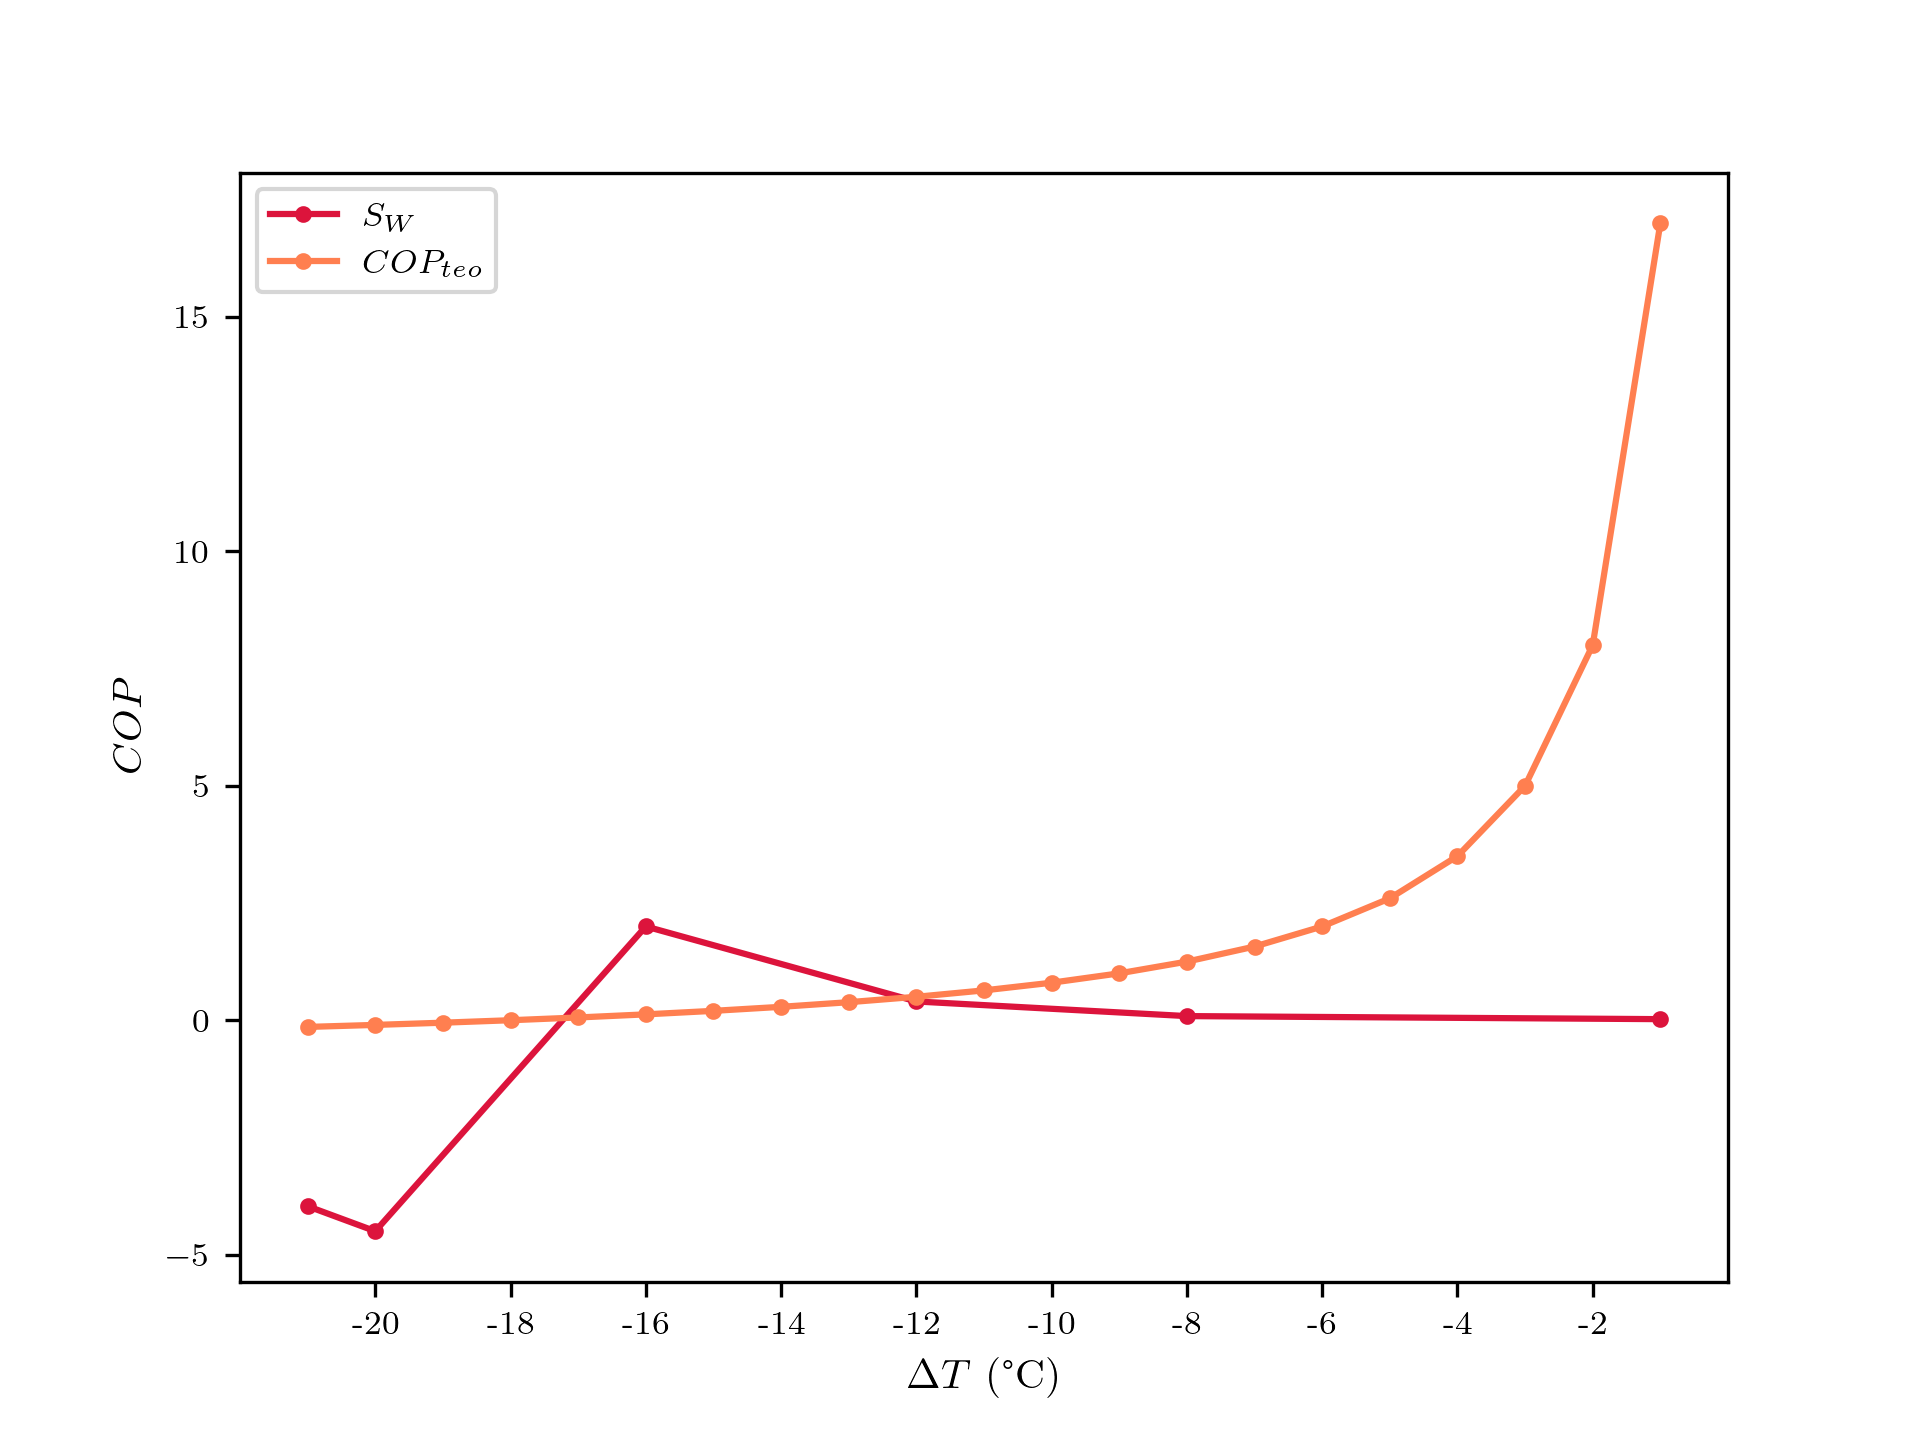
\includegraphics[width = 0.8\linewidth]{img/refri_cops.png}
    \caption{Comparación de los coeficientes de rendimiento.}
    \label{fig:refri_cops}
\end{figure}

